\subsection{Video Representation} \label{subsec:videorepresentation}
\begin{comment}
\textbf{OLD }We represent actions as a sequence of human body poses estimated at each frame.
Our algorithm extracts from RGB-D videos, a feature vector representing body
poses using the methods in \cite{Shotton2011,Chen2010a}.
Specifically,
given a video $D$ with $T$ frames, we extract a feature vector $X = \{x_1,
\ldots, x_T\}$,
where $x_t$ is a set of pose features extracted from the 3D body
configuration estimated at frame $t$.
Our pose features inspired by \cite{Chen2010a} include
relative location between body joints,
angles between limbs and angles between limbs and
planes spanned by body parts.
\end{comment}
%For simplicity, most of the equations are writted considering that each frame is described by a single descriptor. Several works have shown the relevance of including local spatial information to boost recognition \cite{Lazebnik:Schmid:Ponce:2006}.
%Consequently, we account for local information by dividing each body pose at frame $t$ into $R$ spatial region. In our model, we use $R=4$ semantic body regions or parts: right upper body, left upper body, right lower body and left lower body. Each body part contains a limb and several joints, as shown in Fig. \ref{fig:skeleton_limbs_regions}. We write the equations for $R=4$ only when it is necessary to understand the full model.
We represent an input RGB-D video as a sequence of human body poses estimated at each frame. Unlike 
previous work \cite{Escorcia2012,Sung2012}, we do not
compute a global pose descriptor for the entire body.
Instead, we divide the body pose into $R$ fixed spatial regions
and independently compute a pose feature vector for each region.
Fig. \ref{fig:skeleton_limbs_regions} illustrates the case when $R = 4$ that we use in all our 
experiments. Our body pose feature vector consists of the concatenation of two descriptors. At 
frame $t$ and region $r$, a descriptor $x^{g}_{t,r}$ encodes geometric information about the 
spatial configuration of body joints, and a descriptor $x^{m}_{t,r}$ encodes local motion 
information around each body joint position. We present next the 
details behind these descriptors.

%In practice, our algorithm extracts a feature vector for every region and frame
%by combining two descriptors. descriptor that encodes geometric, appearance, and motion 
%cues. 
%Specifically, at frame $t$ a geometric descriptor $x^{s}_{t,r}$ e Additionally, a second 
%descriptor $x^{d}_{t,r}$ encodes the local appearance and motion information around each body 
%joint in a short time interval around frame $t$. Finally, we compute a single descriptor for 
%region $r$ at frame $t$ by concatenation: $x_{t,r} = \begin{bmatrix} x^{s}_{t,r} & x^{d}_{t,r} 
%\end{bmatrix}$.

%We characterize its geometry measuring a set of  angles between selected lines between joints,  
%while for the dynamic 
%descriptor we use Histogram of Optical Flow (HOF) descriptor, computed in 2D image points 
%corresponding to joints in the RGB sequence.

\paragraph{\textbf{Geometric descriptor:}}
Our geometric descriptor is based on the spatial configuration of limbs and body joints, and it is 
inspired by \cite{Chen2010a}.
As illustrated in Fig.~\ref{fig:skeleton_limbs_regions}, we use a body pose model given by the positions of sixteen joints,
which are grouped manually into $R = 4$ fixed regions.
For each region, we compute relative angles among six selected segments, where each segment is a 
line
that connects a pair of joints. We also compute relative angles between each
segment and a plane spanned by sets of three joints. This provides a
total of 18 dimensions (angles) for the geometric descriptor associated to each region.
Table \ref{tab:geometric_relations_for_regions} shows the 6 segments and the plane that define 
each body region. 

%
\begin{figure}[tb]
\begin{center}
\fbox{\rule{0pt}{2in} \rule{0.9\linewidth}{0pt}}
%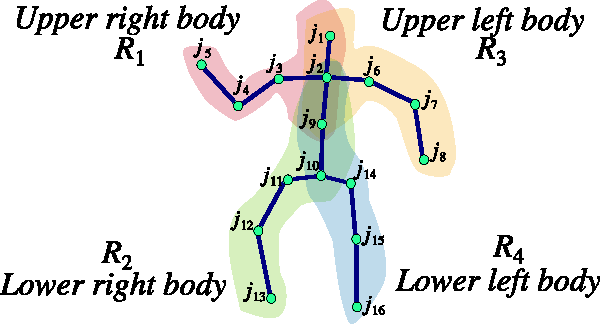
\includegraphics[width=0.95\linewidth]{./fig_joints_limbs_region.pdf}
\end{center}
   \caption{Skeleton representation used for splitting the human body into a set of 
overlapping spatial regions.}
\label{fig:skeleton_limbs_regions}
\end{figure}
%
\begin{table}
\center
%{\small
\begin{tabular}{|l|l|l| }
\hline
Region & Segments & Plane defined by: \\
\hline \hline
$R_1$, $R_3$ & wrist $\rightarrow$ elbow & shoulder \\
& elbow $\rightarrow$ shoulder & elbow \\
& shoulder $\rightarrow$ neck & wrist \\
& wrist $\rightarrow$ shoulder & \\
& wrist $\rightarrow$ head & \\
& neck $\rightarrow$ torso & \\
\hline
$R_2$, $R_4$ & ankle $\rightarrow$ knee &  hip \\
& knee $\rightarrow$ hip & knee \\
& hip $\rightarrow$ hip center & ankle \\
& ankle $\rightarrow$ hip & \\
& ankle$\rightarrow$ torso & \\
& hip center $\rightarrow$ torso & \\
\hline
\end{tabular}
%}
\caption{Segments and planes used by the geometric descriptor to define each body 
region.}
\label{tab:geometric_relations_for_regions}
\end{table}

\paragraph{\textbf{Motion descriptor:}}
While the geometric descriptor captures body pose configurations, it misses to encode
information about the dynamic of each body pose. We argue that motion cues are relevant to 
disambiguate poses that are similar in configuration but move 
differently. Our motion descriptor is based on the trajectory descriptor 
presented in \cite{WangCVPR2011}. While this descriptor also encodes appearance information, our 
experiments indicate that only the part encoding motion through a histogram of optical 
flow (HOF) helps to increase the recognition accuracy of our model. Furthermore, instead of 
calculating a dense descriptor as in \cite{WangCVPR2011}, we only 
encode motion information around each detected body joint location. 
Specifically, following the setup in \cite{WangCVPR2011}, we compute at each joint location a 
HOF using RGB patches centered at the joint location for a 
temporal window of 
15 frames. At each joint location, this produces a 108-dimensional descriptor,  
that we concatenate across all joints to obtain our motion descriptor. Finally, to reduce 
dimensionality, we apply PCA to transform the concatenated descriptor into a 
20-dimensional vector, keeping the dimensionality of our final descriptor 
relatively low.
